\section{Simulation Setup}

To asses performance of different fleet sizes and operational policies, a novel scenario for the city of Zurich, Switzerland was set up for the MATSim transport simulation framework.
 % and a theoretical fleet sizing
%according to \citep{spieser2014toward} is performed.

% Commented to reduce works /sh
%The section is structured as follows:
%First, we give an overview about the used simulation components, second, we specify
%the scenario and finally, we provide fleet sizing results from the theoretical
%methodology presented in \citep{spieser2014toward}.

\subsection{MATSim and AMoD Simulation}

MATSim \citep{Horni2015} is an agent-based transport simulation framework that makes it possible to simulate large numbers of agents representing a real population in a traffic environment. As is the case in real life, each agent has a daily plan with activities intended to be performed for a certain duration and to be finished at a specific time of day. Since these activities take place at different locations in the scenario, agents need to move from activity to activity. By default, MATSim allows simulation of car traffic, public transit and slow modes such as biking or walking. Road-based modes, such as private cars are simulated in a time-step based manner in a queue network with all participants at the same time. This way, congestion can emerge, causing agents to arrive late at their activity locations. While MATSim provides more functionality, e.g. the replanning of agents’ plans to adapt to the traffic conditions that they perceive, only the network simulation is used in this research. However, the framework has been chosen to draw from those possibilities in future research.


An extension to MATSim developed by \citet{horl_abmtrans17} and \citet{towards_testbed}, in combination with the code published in \cite{amodeusBase}, is used to add automated taxis to the set of available travel modes. A virtual dispatcher, for which different algorithms are used in this study, controls a fleet of AVs. Whenever an agent wants to depart from its current activity location by AV, a request is issued to the dispatcher and saved.  The choice which vehicle to send, and when, is completely defined by the dispatching algorithm. Once the vehicle arrives at the customer's location, the pick-up is processed, the AV drives to the destination and finally drops off the customer. Then, the vehicle is available for dispatching again. Alternatively, vehicles can be rebalanced, which means that the dispatcher gives an AV  instructions to drive to a new location. All of this is performed in the MATSim traffic simulation; thus AVs suffer from congestion like any other vehicle. Again, in the present work, this option is disabled and all vehicles are simulated with free-flow speeds because a work-intensive calibration would have to have been performed upfront. Such a simulation will be part of future research.

% Commented out to save words
%It should be noted that AVs drive directly to the locations where agents finish and
%start their activities. So far no mechanism is implemented that would allow them
%to meet at optimized locations, e.g. a high-capacity avenue instead of a small
%alley.

\subsection{Scenario Definition}

For Switzerland, the Microcensus on Mobility and Transport \citep{microcensus} is available, reporting the daily travel patterns of 60,000 survey respondents resident in the country. It is the basis for a readily available agent population of Switzerland, that reproduces the demographic attributes and travel patterns in the country in great detail \citep{ivtbaseline}. Each of the included agents has a detailed travel plan for the simulated day, i.e. where it wants to perform activities and for how long and which mode of transport (car, public transit,bike or walking) should be used to get from one location to the next.

\begin{figure}[h]
\begin{center}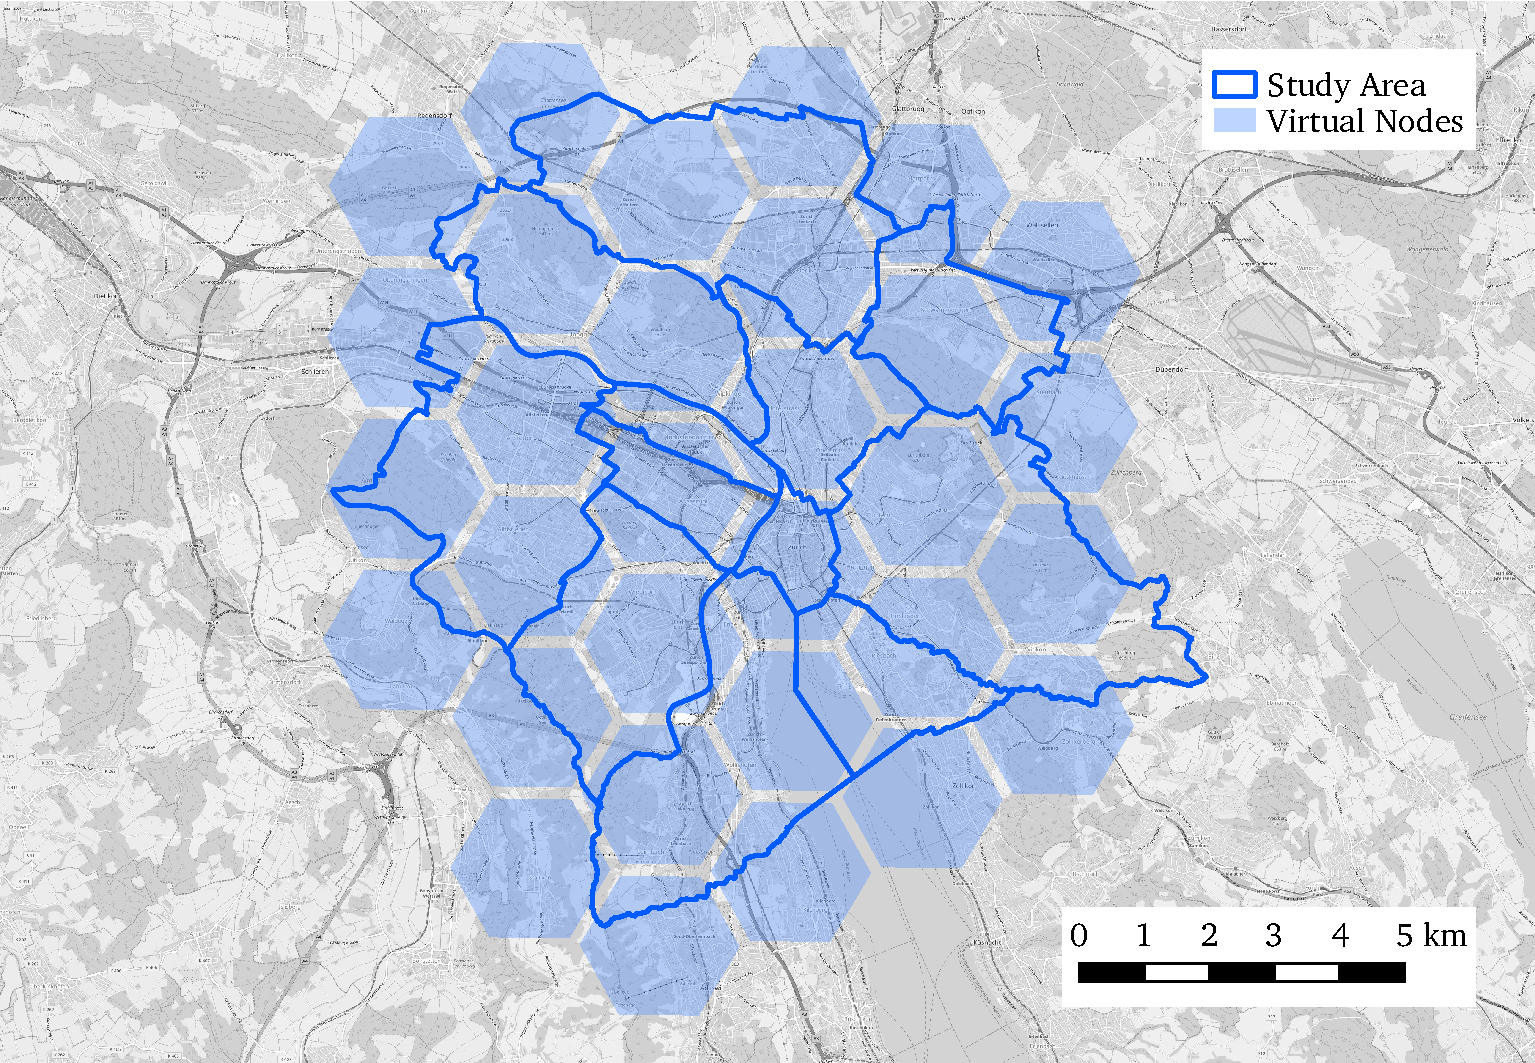
\includegraphics[width=1.0\textwidth]{figures/map.pdf}\end{center}
\caption{AMoD service area covering the 12 districts of Zurich and the nodes of the
virtual network for the rebalancing algorithms. (Map: OpenStreetMap)}
\label{fig:map}
\end{figure}

%Some modifications are applied to this population of around 8 million
%agents to make it suitable for the study at hand. First, a best-response routing
%of the trips of the agents is performed to find all agents that interact
%with a region of a radius of 30km around the city center of Zurich.
%\hl{All agents which do not perform an activity within the study area at any time during the day are removed from the scenario.
%All agents which do not interact with that region (i.e. do not perform an activity within
%the area and do not \hl{enter or leave} the area) are deleted from the population as they do
%not contribute to congestion in the area. Finally, a 10\%
%sample of the remaining agents is created. The rather extensive downscaling becomes necessary for the computationally
%demanding algorithms, given that they need to be performed hundreds of times faster
%than in reality to allow for multiple runs and iterations.

%In order to define the travel demand for the fleet of automated vehicles, agents
%are tagged as whether they are viable for using an automated vehicle or not. Pedestrians
%and cyclists are not simulated at all in this work since they do not contribute to congestion in the current version of the framework.

The operating area of the AMoD service is defined as the 12 districts of Zurich (Figure \ref{fig:map}), which constitute the city core. Travel demand for the AMoD fleet is defined as a ``maximum demand'' case. For this we replace all trips in every agent’s plan that possibly could be served by an automated taxi:


\begin{itemize}
\item In the case of trips that were originally  performed using \textbf{public transit}, we replace the trip with the AMoD mode if both origin and destination of the trip are located within the operating area of the AMoD service.
\item For trips by \textbf{private cars}, the case is more difficult; first we create a set of all possible chains of travel modes with which the agent's plan could be performed and then we filter unfeasible options. These are chains where any AMoD trip would originate or end outside the operating area, but also those where introducing an AMoD trip would violate the continuity constraint for the private vehicle; in an agent’s plan, the car can only be used at a location to where it has previously been driven. After the filtering, the chain with the highest number of remaining AMoD trips for an agent is chosen, so that we have the maximum number of travels by AMoD for each agent.
\item The slow modes (biking and walking) are never replaced by the AMoD mode.
\end{itemize}

In conclusion, around 8 million agents of the synthetic Swiss population are reduced to about 137,000 agents entering, leaving, or within the study area at any time during the day. These agents’ plans contain 363,503 trips to be served by AVs.
